\subsection{笛卡尔方块的复合}

命题 7. --- 设

\[
\begin{array}{c} \mathrm {X^ {\prime\prime}} \xrightarrow {g ^ {\prime}} \mathrm {X^ {\prime}} \\ \Big \downarrow_ {p ^ {\prime \prime}} \\ \mathrm {B^ {\prime\prime}} \xrightarrow {g} \mathrm {B^ {\prime}} \end{array}\tag{12}
\]

和

\begin{enumerate}
\def\labelenumi{(\arabic{enumi})}
\setcounter{enumi}{12}
\tightlist
\item
\end{enumerate}

\pandocbounded{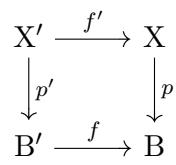
\includegraphics[keepaspectratio]{images/part001_4552bd62.jpg}}

为两个交换方块；考虑方块

\begin{enumerate}
\def\labelenumi{(\arabic{enumi})}
\setcounter{enumi}{13}
\tightlist
\item
\end{enumerate}

\pandocbounded{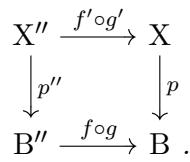
\includegraphics[keepaspectratio]{images/part001_1603e4c4.jpg}}

它是交换的。若方块 (12) 与 (13) 都是笛卡尔的，则方块 (14) 亦然。若方块 (13) 与 (14) 都是笛卡尔的，则方块 (12) 亦然。

方块 (14) 是交换的，因为我们有 \(p \circ f' \circ g' = f \circ p' \circ g' = f \circ g \circ p''\) 。用 \(h' : X'' \to B'' \times_{B'} X'\) 、\(h : X' \to B' \times_{B} X\) 与 \(h'' : X'' \to B'' \times_{B} X\) 表示分别由交换方块 (12)、(13) 与 (14) 得到的典型连续映射。此外，用

\[
j \colon \mathrm{B} ^ {\prime \prime} \times_ {\mathrm{B}} \mathrm{X} \rightarrow \mathrm{B} ^ {\prime \prime} \times_ {\mathrm{B} ^ {\prime}} (\mathrm{B} ^ {\prime} \times_ {\mathrm{B}} \mathrm{X})
\]

表示把 \((b'', x)\) 映为 \((b'', g(b''), x)\) 的连续映射。它是一个同胚，并且有 \(j \circ h'' = (\mathrm{Id}_{\mathrm{B}''} \times_{\mathrm{B}} h) \circ h'\) 。

设方块 (13) 是笛卡尔的。于是 h 是一个同胚 (I, p. 8, prop 2)，从而映射 \(Id_{B''} \times_{B} h\) 是一个同胚，并且 \(h''\) 是同胚当且仅当 \(h'\) 是同胚。这就是说，方块 (12) 是笛卡尔的当且仅当方块 (14) 是笛卡尔的 (loc. cit.)。

采用命题 7 中的记号，有时称方块 (14) 为方块 (13) 与 (12) 的复合方块。第一个断言表明：两个笛卡尔方块的复合是笛卡尔的。特别地，B''-空间 \(g^{*}(f^{*}(\mathrm{X}))\) 与 \((f \circ g)^{*}(\mathrm{X})\) 是同构的。

\pandocbounded{
\includegraphics[keepaspectratio]{images/part001_52f28a70.jpg}}

注. --- 1) 可能发生这样的情形：方块 (12) 与 (14) 都是笛卡尔的，而方块 (13) 却不是 (I, p. 139, exerc. 2)。

\begin{enumerate}
\def\labelenumi{\arabic{enumi})}
\setcounter{enumi}{1}
\tightlist
\item
  设 \(p \colon \mathrm{X} \to \mathrm{B}\) 与 \(f \colon \mathrm{B}' \to \mathrm{B}\) 为连续映射。映射 \(g \colon \mathrm{B}' \to \mathrm{B}' \times \mathrm{B}\) （由 \(g(b') = (b', f(b'))\) 定义）是从 \(\mathrm{B}'\) 到图像 \(\mathrm{G}\) （映射 \(f\) 的）上的一个同胚 (TG, I, p. 25, cor. 2)，而纤维积 \(\mathrm{B}' \times_{\mathrm{B}} \mathrm{X}\) 可以等同 (I, p. 6) 于 \(\mathrm{B}' \times \mathrm{X}\) 的一个子空间，即 \(\mathrm{G}\) 在映射 \(\mathrm{Id}_{\mathrm{B}'} \times p \colon \mathrm{B}' \times \mathrm{X} \to \mathrm{B}' \times \mathrm{B}\) 下的原像。由 I, p. 10 的例与命题 5 的推论 1 (I, p. 11)，方块
\end{enumerate}

\[
\begin{array}{c c} \mathrm {B^ {\prime}} \times_ {\mathrm{B}} \mathrm{X} \xrightarrow {i} \mathrm {B^ {\prime}} \times \mathrm{X} & \mathrm {B^ {\prime}} \times \mathrm{X} \xrightarrow {\mathrm{pr} _ {2}} \mathrm{X} \\ \Biggl \downarrow \mathrm{pr} _ {1} & \Biggl \downarrow \mathrm{Id} _ {\mathrm {B^ {\prime}}} \times p \\ \mathrm {B^ {\prime}} \xrightarrow {g} \mathrm {B^ {\prime}} \times \mathrm{B} & \text {et} \end{array} \qquad \qquad \begin{array}{c c} \mathrm {B ^ {\prime}} \times \mathrm{X} \xrightarrow {\mathrm{pr} _ {2}} \mathrm{X} \\ \Biggl \downarrow \mathrm{Id} _ {\mathrm {B^ {\prime}}} \times p & \Biggl \downarrow p \\ \mathrm {B^ {\prime}} \times \mathrm{B} \xrightarrow {\mathrm{pr} _ {2}} \mathrm{B} & \end{array}
\]

（其中 i 表示典型单射）都是笛卡尔的，而笛卡尔方块

\[
\begin{array}{c} \mathrm{B} ^ {\prime} \times_ {\mathrm{B}} \mathrm{X} \xrightarrow {\mathrm{pr} _ {2}} \mathrm{X} \\ \Big \downarrow \mathrm{pr} _ {1} \\ \mathrm{B} ^ {\prime} \xrightarrow {f} \mathrm{B} \end{array}
\]

是它们的复合。换句话说，每个笛卡尔方块都等同于一个由取积得到的笛卡尔方块 (I, p. 11, 命题 5 的推论 1, 方块 (8)) 与一个由过渡到子空间得到的笛卡尔方块 (I, p. 10, 例, 方块 (5)) 的复合方块。

\begin{enumerate}
\def\labelenumi{\arabic{enumi})}
\setcounter{enumi}{2}
\tightlist
\item
  设
\end{enumerate}

\[
\begin{array}{c} \mathrm{X} _ {1} \xrightarrow {g _ {1}} \mathrm{X} \\ \Biggl \downarrow p _ {1} \\ \mathrm{B} _ {1} \xrightarrow {f _ {1}} \mathrm{B} \end{array}\tag{15}
\]

和

\[
\begin{array}{c} \mathrm{X} _ {2} \xrightarrow {g _ {2}} \mathrm{X} \\ \Biggl \downarrow p _ {2} \\ \mathrm{B} _ {2} \xrightarrow {f _ {2}} \mathrm{B} \end{array}\tag{16}
\]

  设

\[
\begin{array}{c} \mathrm{X} _ {1} \times_ {\mathrm{X}} \mathrm{X} _ {2} \xrightarrow {g} \mathrm{X} \\ \Big \downarrow^ {p ^ {\prime}} \\ \mathrm{B} _ {1} \times_ {\mathrm{B}} \mathrm{B} _ {2} \xrightarrow {f} \mathrm{B} \end{array}\tag{17}
\]

其中 \(f\) （相应地，\(g\) ）是在纤维积 \(\mathrm{B}_{1} \times_{\mathrm{B}} \mathrm{B}_{2}\) （相应地，纤维积 \(\mathrm{X}_{1} \times_{\mathrm{X}} \mathrm{X}_{2}\) ）上定义 B-空间（相应地，X-空间）结构的映射，而 \(p'\) 是由 \(p_{1} \times p_{2}\) 过渡到子空间所诱导的映射。它是笛卡尔的 (I, p. 13, 命题 5 的推论 2)。

现在考虑下面两个交换方块：

\[
\begin{array}{c c} \mathrm{X} _ {1} \times_ {\mathrm{X}} \mathrm{X} _ {2} \xrightarrow {\operatorname{pr} _ {1}} \mathrm{X} _ {1} & \mathrm{X} _ {1} \times_ {\mathrm{X}} \mathrm{X} _ {2} \xrightarrow {\operatorname{pr} _ {2}} \mathrm{X} _ {2} \\ \Biggl \downarrow p ^ {\prime} & \text {and} \\ \mathrm{B} _ {1} \times_ {\mathrm{B}} \mathrm{B} _ {2} \xrightarrow {\operatorname{pr} _ {1}} \mathrm{B} _ {1} & \mathrm{(19)} \\ & \mathrm{B} _ {1} \times_ {\mathrm{B}} \mathrm{B} _ {2} \xrightarrow {\operatorname{pr} _ {2}} \mathrm{B} _ {2}. \end{array}\tag{18}
\]

方块 (17) 由方块 (15) 与 (18) 复合而成，也由方块 (16) 与 (19) 复合而成。由命题 7，方块 (18) 与 (19) 都是笛卡尔的。

